\documentclass{beamer}
\usepackage[english]{babel}
\usepackage[utf8]{inputenc}
\usepackage{verbatim}
\usepackage{graphicx}

\begin{document}

\title{Telepathy Skykit}
\author{Maksim Melnikau (max\_posedon)}
\institute{Linux Mobile hobbyist\\World of Tanks developer}
\date{\today}
\frame{\titlepage}

\section{Instant Messaging}
\frame{
    \Large{Instant Messaging in Linux} \pause \Huge{SUCKS}
}

\frame{
    \frametitle{Facebook Web UI}
    \begin{columns}
    
    \begin{column}{0.5\textwidth}
    \begin{figure}[htb]
    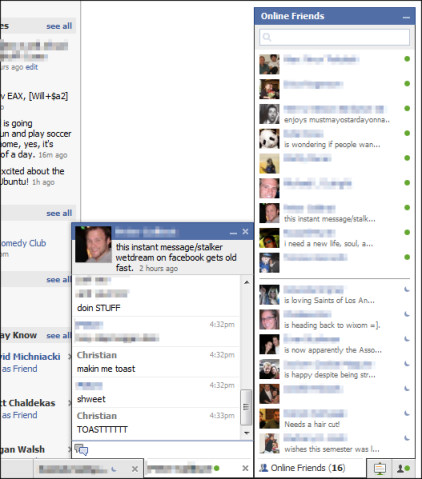
\includegraphics[width=\textwidth]{fbchat.jpg}
    \end{figure}
    \end{column}

    \pause

    \begin{column}{0.5\textwidth}
    \begin{itemize}
    \item no audio
    \item no video
    \item no groups
    \item facebook accounts only
    \end{itemize}
    \end{column}

    \end{columns}
}

\frame{
    \frametitle{Google Talk Web UI}
    \begin{columns}

    \begin{column}{0.5\textwidth}
    \begin{figure}[htb]
    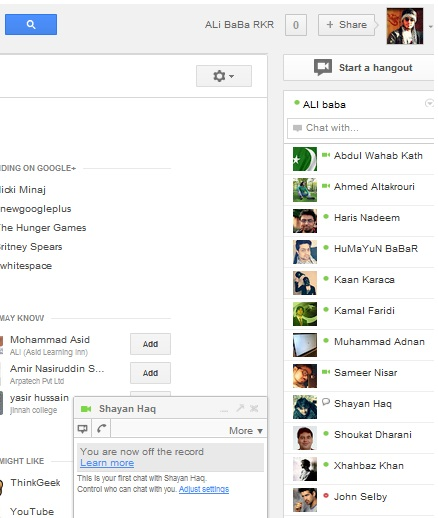
\includegraphics[width=\textwidth]{gpchat.jpg}
    \end{figure}
    \end{column}

    \pause

    \begin{column}{0.5\textwidth}
    \begin{itemize}
    \item Google accounts only
    \end{itemize}
    \end{column}

    \end{columns}
}

\frame{
    \frametitle{Skype}
    \begin{columns}

    \begin{column}{0.5\textwidth}
    \begin{figure}[htb]
    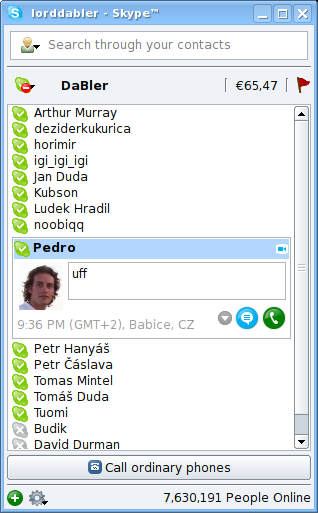
\includegraphics[width=0.8\textwidth]{skypechat.png}
    \end{figure}
    \end{column}

    \pause

    \begin{column}{0.5\textwidth}
    \begin{itemize}
    \item awful L\&F
    \item no PIM/DE integration
    \item x86-desktop only on Linux
    \end{itemize}
    \end{column}

    \end{columns}
}

\frame{
    \frametitle{Pidgin}
    \begin{columns}

    \begin{column}{0.5\textwidth}
    \begin{figure}[htb]
    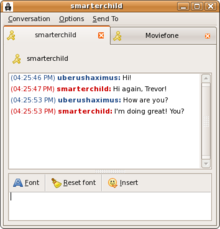
\includegraphics[width=\textwidth]{pidginchat.png}
    \end{figure}
    \end{column}

    \pause

    \begin{column}{0.5\textwidth}
    \begin{itemize}
    \item no audio
    \item no video
    \item no PIM/DE integration
    \end{itemize}
    \end{column}

    \end{columns}
}

\frame{
    \frametitle{Cool Example: \uncover<2>{n900}}
    \begin{columns}

    \uncover<2>{
    \begin{column}{0.5\textwidth}
    \begin{figure}[htb]
    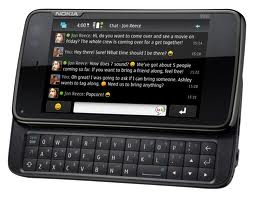
\includegraphics[width=\textwidth]{n900.jpg}
    \end{figure}
    \end{column}
    }

    \begin{column}{0.5\textwidth}
    \begin{itemize}
    \item audio 
    \item video
    \item PIM/DE integration
    \item multiple protocols
    \item touch interface
    \end{itemize}
    \end{column}

    \end{columns}
}

\section{telepathy}
\frame{
    \begin{figure}[htb]
    
\includegraphics[width=\textwidth]{telepathy.png}
    \end{figure}
}

\frame{
    \frametitle{The Unix Way}
    \begin{block}{Do \alt<1-3>{\temporal<2>{one}{two}{six}}{twelve} thing\alt<1>{}{s} and do it well\only<4>{?}}

    \begin{itemize}
    \item<1> Instant Messaging
    \end{itemize}

    \begin{columns}

    \begin{column}{0.5\textwidth}
    \begin{itemize}
    \item<2> User Interface
    \item<3-4> Contact List
    \item<3-4> Chat
    \item<3-4> Logging
    \item<4> File Transfer
    \item<4> Voice Call
    \item<4> Tubes
    \end{itemize}
    \end{column}

    \begin{column}{0.5\textwidth}
    \begin{itemize}
    \item<2> Protocol
    \item<3-4> AIM
    \item<3-4> MSN
    \item<3-4> XMPP
    \item<4> SIP
    \item<4> ICQ
    \item<4> IRC
    \end{itemize}
    \end{column}

    \end{columns}
    \end{block}
}

\frame{
    \frametitle{Telepathy Architecture}
    
    \begin{itemize}
    \item move away from the monolithic client
    \item split stuff into separate processes
    \item run protocols as services
    \item create a standard DBUS API
    \end{itemize}

    \pause

    \begin{figure}[htb]
    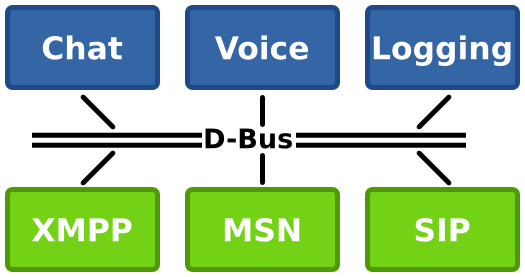
\includegraphics[width=0.8\textwidth]{tao.png}
    \end{figure}
}

\frame{
    \frametitle{KDE Telepathy}
    \begin{figure}[htb]
    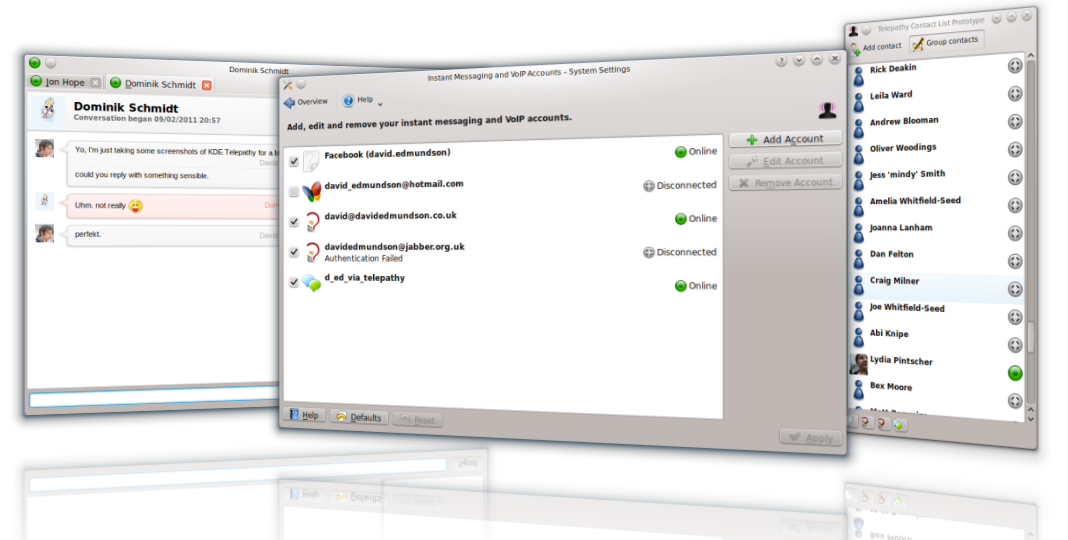
\includegraphics[width=\textwidth]{ktp.jpg}
    \end{figure}
}

\frame{
    \frametitle{Empathy}
    \begin{figure}[htb]
    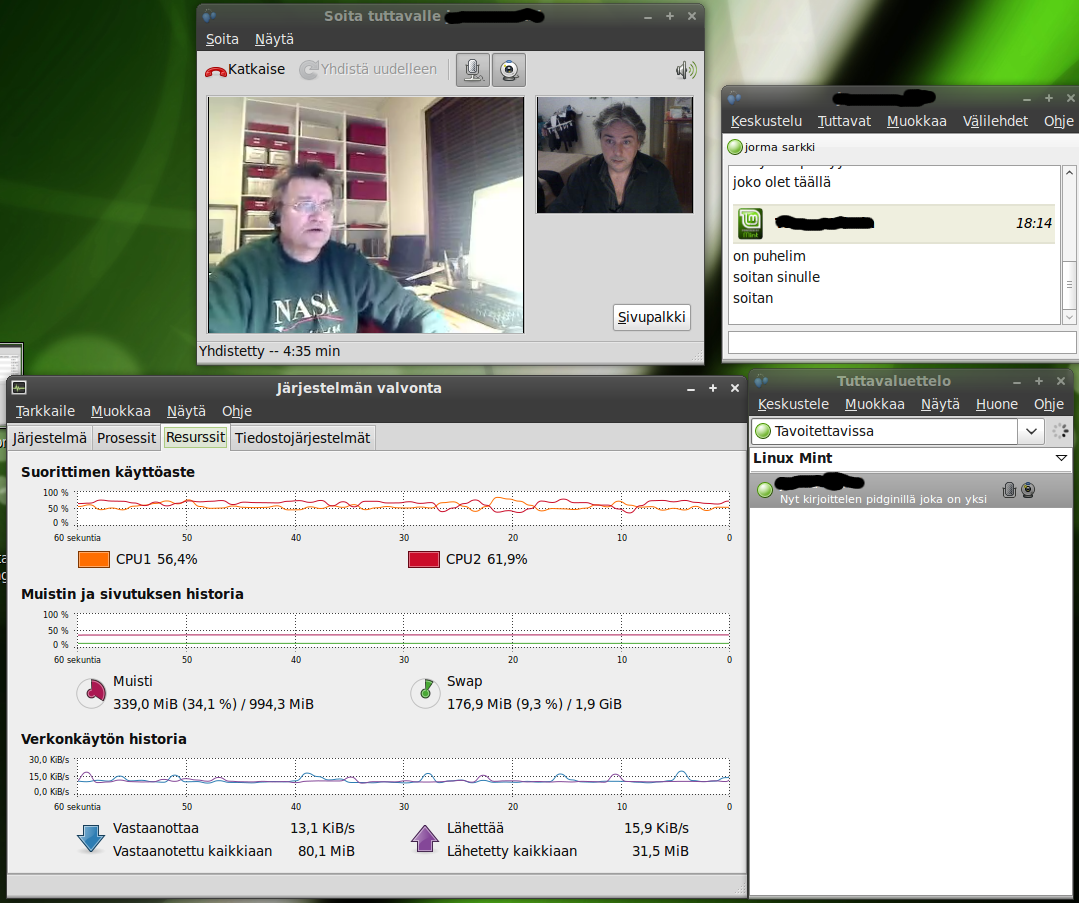
\includegraphics[width=\textwidth]{empathy.png}
    \end{figure}
}

\section{Skypekit}
\frame{
    \frametitle{Skype\uncover<2>{kit}}
    
    \pause

    \begin{figure}[htb]
    
\includegraphics[width=0.8\textwidth]{skypekit.jpg}
    \end{figure}

    \begin{itemize}
    \item headless version of Skype
    \item different OS
    \item different arches for Linux
    \item audio, video, ...
    \item not free (\$5 for developer license)
    \end{itemize}
}

\section{telepathy-skykit}
\frame{
    \frametitle{Telepathy Skykit}

    \begin{columns}

    \begin{column}{0.5\textwidth}
    \begin{figure}[htb]
    
\includegraphics[width=\textwidth]{skykit.png}
    \end{figure}
    \end{column}

    \begin{column}{0.5\textwidth}
    \begin{itemize}
    \item protocol service
    \item connection manager
    \item telepathy based
    \item skypekit based
    \item python
    \item telepathy-python
    \item open source
    \item no license (now)
    \end{itemize}
    \end{column}
    
    \end{columns}
}

\frame{
    \frametitle{Telepathy Skykit}
    \begin{columns}

    \begin{column}{0.5\textwidth}
    \begin{figure}[htb]
    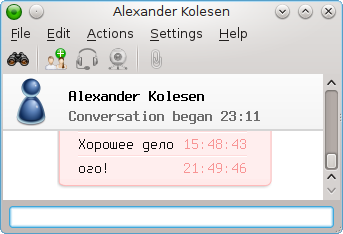
\includegraphics[width=0.9\textwidth]{ktpskype.png}
    \end{figure}
    \end{column}
    
    \pause

    \begin{column}{0.25\textwidth}
    \begin{block}{Supports}
    \begin{itemize}
    \item presence
    \item contact list
    \item 1:1 chat
    \item avatar
    \item vcard
    \end{itemize}
    \end{block}
    \end{column}
    
    \pause

    \begin{column}{0.25\textwidth}
    \begin{block}{Future plans}
    \begin{itemize}
    \item MUC
    \item file transfer
    \item audio
    \item video
    \item ...
    \end{itemize}
    \end{block}
    \end{column}
    
    \end{columns}
}

\frame{
    \frametitle{More Info}
    \begin{itemize}
    \item Maksim Melnikau (max\_posedon)
    \item email: maxposedon@gmail.com
    \item https://github.com/max-posedon/telepathy-skykit
    \item https://github.com/max-posedon/telepathy-python
    \item http://telepathy.freedesktop.org/wiki/
    \item https://dev.skype.com/skypekit
    \item https://github.com/max-posedon/talk-telepathy-skykit
    \end{itemize}
}

\end{document}
